\documentclass[12pt, twoside]{article}
\usepackage[letterpaper, margin=1in, headsep=0.5in]{geometry}
\usepackage[english]{babel}
\usepackage[utf8]{inputenc}
\usepackage{amsmath}
\usepackage{amsfonts}
\usepackage{amssymb}
\usepackage{tikz}
%\usetikzlibrary{quotes, angles}

\usepackage{graphicx}
\usepackage{enumitem}
\usepackage{multicol}

\usepackage{fancyhdr}
\pagestyle{fancy}
\fancyhf{}
\renewcommand{\headrulewidth}{0pt} % disable the underline of the header

\fancyhead[RE]{\thepage}
\fancyhead[RO]{\thepage \\ Name: \hspace{3cm}}
\fancyhead[L]{BECA / Dr. Huson / 10th Grade Geometry\\* 15 March 2019}

\begin{document}
\subsubsection*{8-9 Do Now Quiz: Similar triangles, dilation ratios}
 \begin{enumerate}

  \begin{multicols}{2}
  [\item A translation maps triangle $PQR$ onto triangle $STU$.] \vspace{0.5cm}
    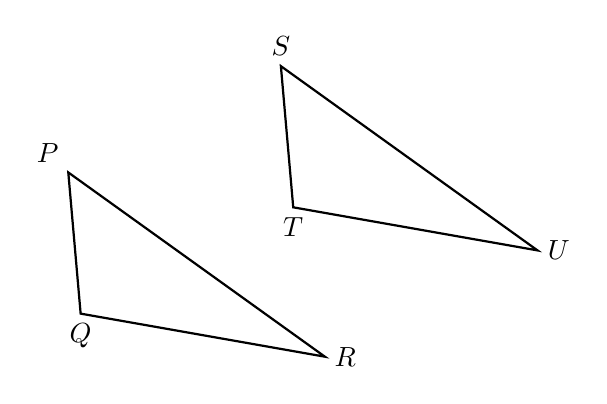
\begin{tikzpicture}[scale=0.9]
      \coordinate [label=above left:$P$](A) at (95:2);
      \coordinate [label=below:$Q$](B) at (0, 0);
      \coordinate [label=right:$R$](C) at (-10:3.5);
      \draw [thick] (A)--(B)--(C)--cycle;

      \draw [thick, xshift=3cm, yshift=1.5cm] (95:2) node[above]{$S$}--
      (0,0) node[below]{$T$}--
      (-10:3.5) node[right]{$U$}--cycle;
    \end{tikzpicture}\\
    Write each corresponding object.
    \begin{enumerate}
      \item $Q \rightarrow$ \rule{2cm}{0.15mm}
      \item $\angle QRP \cong$ \rule{2cm}{0.15mm}
      \item \rule{2cm}{0.15mm} $\cong \overline {ST}$
      \item Justify $\triangle PQR \cong \triangle STU$. Use the words ``rigid motion" and ``$SSS \triangle \cong$."
    \end{enumerate}
  \end{multicols}  \vspace{2cm}

  \item Given $\triangle JKL \sim \triangle MNO$. $m\angle K = 40^\circ$ and $m\angle M = 100^\circ$.\\
  Find the measure of $\angle L$. \vspace{3cm}

 \item Triangle $ABC$ is dilated with a scale factor of $k$ centered at $A$, yielding $\triangle ADE$, as shown. Given $AB=8$, $BC=10$, $AC=12$, and $DE=15$. \\[0.25cm] Find $AD$, $CE$, and $k$ (the scale factor). \vspace{0.5cm}
 \begin{center}
     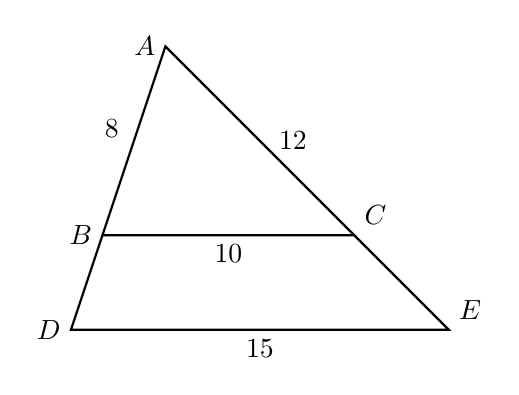
\begin{tikzpicture}[scale=0.4]
       \draw [thick]
       (0,0)node[left]{$B$}--
       (8,0)node[above right]{$C$}--
       (2,6)node[left]{$A$}--cycle;
       \draw [thick]
       (0,0)--
       (-1,-3)node[left]{$D$}--
       (11,-3)node[above right]{$E$}--(8,0);
       \node at (4,0)[below]{$10$};
       \node at (5.3, 3)[right]{$12$};
       \node at (0.3, 2.8)[above]{$8$};
       \node at (5,-3)[below]{$15$};
     \end{tikzpicture}
   \end{center}

\newpage

 \item What transformation maps $\triangle ABC$ onto $\triangle DEC$, shown below? Fully specify the transformation. \\[0.25cm]

     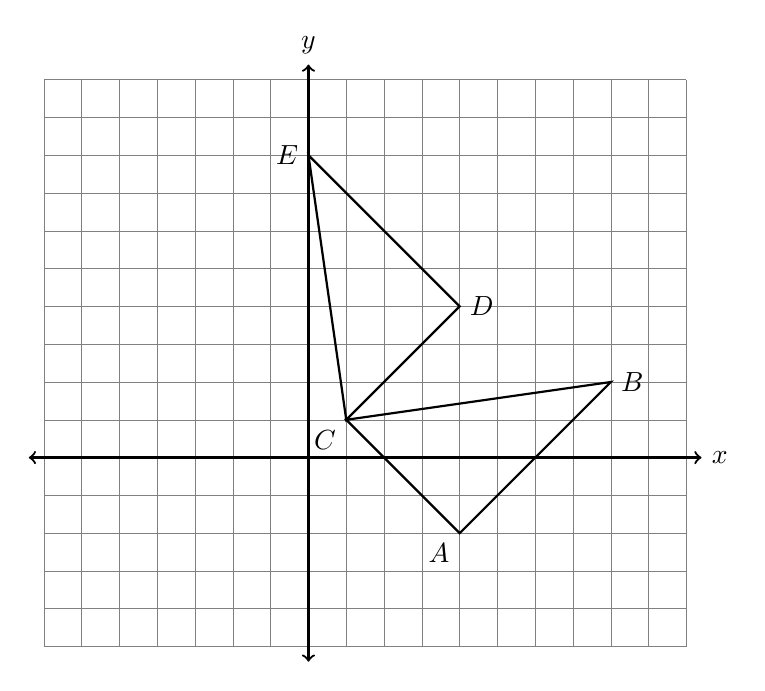
\begin{tikzpicture}[scale=.48]
       \draw [help lines] (-7,-5) grid (10,10);
       \draw [thick, <->] (-7.4,0) -- (10.4,0) node [right] {$x$};
       \draw [thick, <->] (0,-5.4)--(0,10.4) node [above] {$y$};

       \draw [thick]
       (4,-2) node[below left] {$A$}--
       (8,2) node[right] {$B$}--
       (1,1) node[below left] {$C$}--cycle;

       \draw [thick]
       (4,4) node[right] {$D$}--
       (0,8) node[left] {$E$}--
       (1,1) --cycle;

     \end{tikzpicture} \vspace{2cm}

     \item What is the smallest non-zero angle of rotation about its center that would map hexagon $ABCDEF$ onto itself? \vspace{0.5cm}
     \begin{center}
         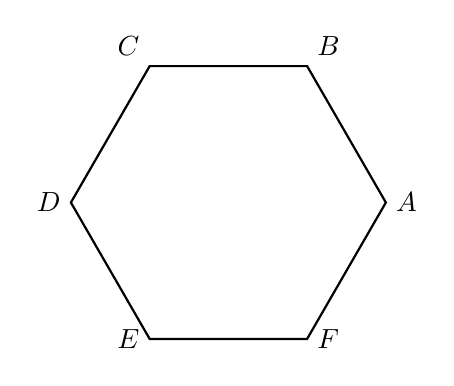
\begin{tikzpicture}%[scale=.48]
           \draw [thick]
           (0:2) node[right] {$A$}--
           (60:2) node[above right] {$B$}--
           (120:2) node[above left] {$C$} --
           (180:2) node[left] {$D$}--
           (240:2) node[left] {$E$}--
           (300:2) node[right] {$F$}--cycle;
         \end{tikzpicture}
       \end{center}
\end{enumerate}

\newpage

\subsubsection*{8-9 Homework: Similar triangles, dilation, symmetry}
 \begin{enumerate}

 \item Given $\triangle ABP$ and $\triangle JKP$ as shown below. $\overline{AB} \parallel \overline{JK}$. $AP=7$, $JP=14$, and $JK=18$. Find $AB$.
 \begin{center}
   \begin{tikzpicture}[scale=1.4]
       \draw [thick]
         (0.25,-1)node[right]{$B$}--
         (-0.5,2)node[left]{$K$}--
         (4,0)node[right]{$J$}--
         (0,0)node[above right]{$P$}--
         (-2,0)node[left]{$A$}--cycle;
     \end{tikzpicture}
     \end{center}

     \vspace{2cm}

 \item Triangle $ABC$ is dilated with a factor of $\frac{5}{4}$ centered at $A$, yielding $\triangle ADE$, as shown. Given $AB=8$, $BC=12$, and $AC=14$. \\[0.25cm] Find $BD$, $AE$, and $DE$. \vspace{1cm}
 \begin{center}
     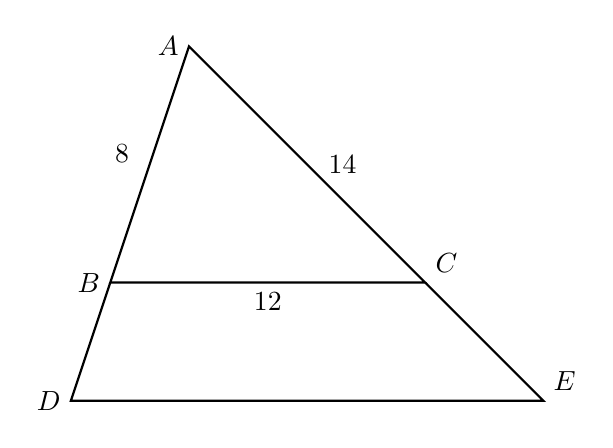
\begin{tikzpicture}[scale=0.5]
       \draw [thick]
       (0,0)node[left]{$B$}--
       (8,0)node[above right]{$C$}--
       (2,6)node[left]{$A$}--cycle;
       \draw [thick]
       (0,0)--
       (-1,-3)node[left]{$D$}--
       (11,-3)node[above right]{$E$}--(8,0);
       \node at (4,0)[below]{$12$};
       \node at (5.3, 3)[right]{$14$};
       \node at (0.3, 2.8)[above]{$8$};
     \end{tikzpicture}
   \end{center}



   \newpage
   \item What is the smallest non-zero angle of rotation about its center that would map octagon $ABCDEFGH$ onto itself? \vspace{0.25cm}
   \begin{center}
       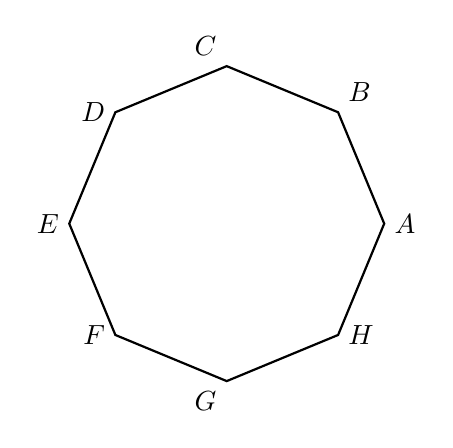
\begin{tikzpicture}%[scale=.48]
         \draw [thick]
         (0:2) node[right] {$A$}--
         (45:2) node[above right] {$B$}--
         (90:2) node[above left] {$C$} --
         (135:2) node[left] {$D$}--
         (180:2) node[left] {$E$}--
         (225:2) node[left] {$F$}--
         (270:2) node[below left] {$G$}--
         (315:2) node[right] {$H$}--cycle;
       \end{tikzpicture}
     \end{center}



    \item The vertices of $\triangle JKL$ have the coordinates $J(-4,-2)$, $K(-1,-1)$, and $L(-2,3)$, as shown below. \\[0.5cm]
    Apply a translation of $(x,y) \rightarrow (x-3, y+2)$ to $\triangle JKL$ and then reflect the image across the $y$-axis. Draw both images $\triangle J'K'L'$ and $\triangle J''K''L''$ on the set of axes below, labeling the vertices.  \vspace{3cm}
    \begin{center}
      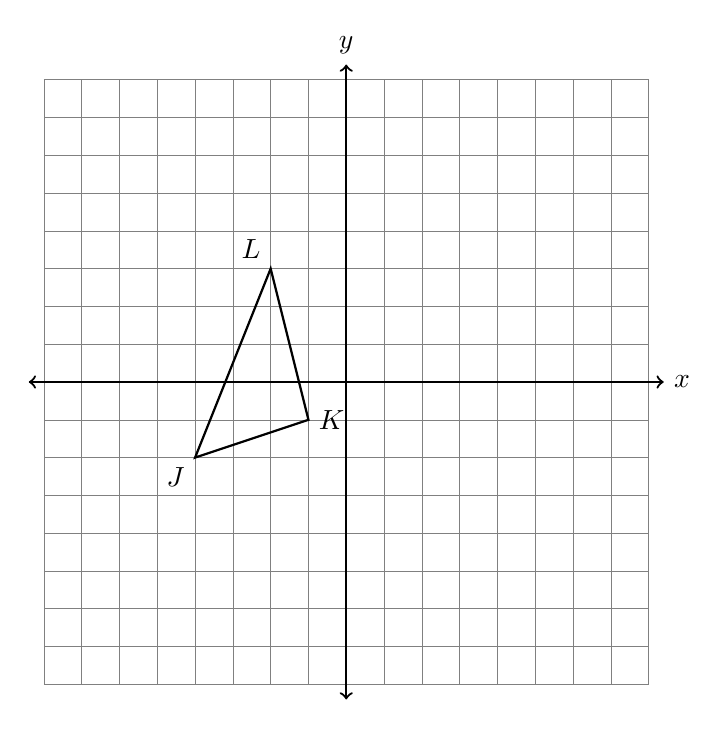
\begin{tikzpicture}[scale=.48]
        \draw [help lines] (-8,-8) grid (8,8);
        \draw [thick, <->] (-8.4,0) -- (8.4,0) node [right] {$x$};
        \draw [thick, <->] (0,-8.4)--(0,8.4) node [above] {$y$};

        \draw [thick]
        (-4,-2) node[below left] {$J$}--
        (-1,-1) node[right] {$K$}--
        (-2,3) node[above left] {$L$}--
        cycle;
      \end{tikzpicture}
    \end{center}



\newpage


\item Given $\triangle ABP$ and $\triangle JKP$ as shown below. $\overline{AB} \parallel \overline{JK}$ with $AB=5$, $PA=4$, $PB=2$, and $PK=5$.\\[0.25cm]
Find $PJ$ and $JK$.\\[0.5cm]
  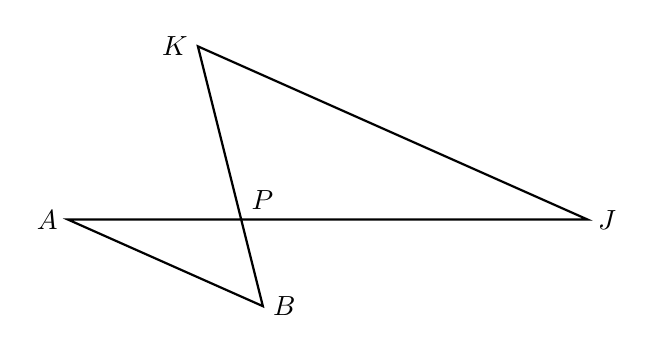
\begin{tikzpicture}[scale=1.1]
      \draw [thick]
        (0.25,-1)node[right]{$B$}--
        (-0.5,2)node[left]{$K$}--
        (4,0)node[right]{$J$}--
        (0,0)node[above right]{$P$}--
        (-2,0)node[left]{$A$}--cycle;
    \end{tikzpicture}
    \vspace{3cm}


    \item Triangle $ADE$ and its midline $\overline{BC}$ are drawn, with $B$ the midpoint of $\overline{AD}$ and $C$ the midpoint of $\overline{AE}$. The two medians $\overline{AE}$ and $\overline{AE}$ are drawn, as shown, intersecting in point $F$, the centroid.\\[0.25cm]
    $\triangle FCB \sim \triangle FDE$ with scale factor $k=2$.\\[0.25cm]
    Given $BC=9$, find $DE$. \\[0.25cm] Given $BF=5$, find $FE$. %\vspace{1cm}
    \begin{center}
        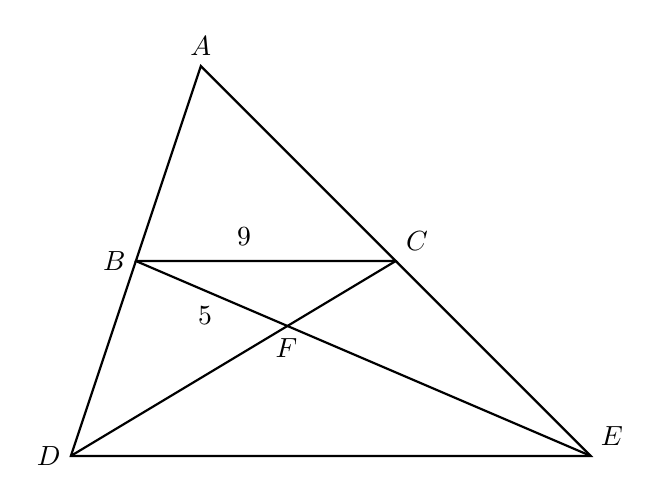
\begin{tikzpicture}[scale=0.55]
          \draw [thick]
          (0.5,1.5)node[left]{$B$}--
          (6.5,1.5)node[above right]{$C$}--
          (2,6)node[above]{$A$}--cycle;
          \draw [thick]
          (0.5,1.5)--
          (-1,-3)node[left]{$D$}--
          (11,-3)node[above right]{$E$}--(6.5,1.5);
          \draw [thick] (0.5,1.5)--(11,-3);
          \draw [thick] (6.5,1.5)--(-1,-3);
          \node at (3,2.5)[below]{$9$};
          \node at (3.5, -0.5)[right]{$F$};
          \node at (2.1, -0.2)[above]{$5$};
          %\node at (-0.7, -1)[above]{$5$};
        \end{tikzpicture}
      \end{center} \vspace{1cm}

  \item Using a compass and straightedge, construct the perpendicular bisector of $\overline{BB'}$  \\[0.25cm]
  What transformation has been applied to map $\triangle ABC$ on to $\triangle A'B'C'$? \vspace{2cm}
      \begin{center}
      \begin{tikzpicture}%[scale=.48]
        %\draw [thick, <->] (-7.4,0) -- (10.4,0) node [right] {$x$};
        %\draw [thick, <->] (0,-6.4)--(0,10.4) node [above] {$y$};

        \draw [thick]
        (5,-1) node[below left] {$A$}--
        (8,2) node[right] {$B$}--
        (1,0) node[below left] {$C$}--cycle;

        \draw [thick]
        (-1,5) node[right] {$A'$}--
        (2,8) node[above] {$B'$}--
        (0,1) node[below left] {$C'$}--cycle;

      \end{tikzpicture}
    \end{center}

\end{enumerate}
\end{document}
